%iffalse
\documentclass[journal]{IEEEtran}
\usepackage[a5paper, margin=10mm]{geometry}
%\usepackage{lmodern} % Ensure lmodern is loaded for pdflatex
\usepackage{tfrupee} % Include tfrupee package


\setlength{\headheight}{1cm} % Set the height of the header box
\setlength{\headsep}{0mm}     % Set the distance between the header box and the top of the text


%\usepackage[a5paper, top=10mm, bottom=10mm, left=10mm, right=10mm]{geometry}

%
\setlength{\intextsep}{10pt} % Space between text and floats

\makeindex


\usepackage{cite}
\usepackage{amsmath,amssymb,amsfonts,amsthm}
\usepackage{algorithmic}
\usepackage{graphicx}
\usepackage{textcomp}
\usepackage{xcolor}
\usepackage{txfonts}
\usepackage{listings}
\usepackage{enumitem}
\usepackage{mathtools}
\usepackage{gensymb}
\usepackage{comment}
\usepackage[breaklinks=true]{hyperref}
\usepackage{tkz-euclide} 
\usepackage{listings}
\usepackage{multicol}
\usepackage{xparse}
\usepackage{gvv}
%\def\inputGnumericTable{}                                 
\usepackage[latin1]{inputenc}                                
\usepackage{color}                                            
\usepackage{array}                                            
\usepackage{longtable}                                       
\usepackage{calc}                                             
\usepackage{multirow}                                         
\usepackage{hhline}                                           
\usepackage{ifthen}  
\usepackage{wrapfig}
\usepackage{lscape}
\usepackage{tabularx}
\usepackage{array}
\usepackage{float}
\usepackage[justification=centering]{caption}


\newtheorem{theorem}{Theorem}[section]
\newtheorem{problem}{Problem}
\newtheorem{proposition}{Proposition}[section]
\newtheorem{lemma}{Lemma}[section]
\newtheorem{corollary}[theorem]{Corollary}
\newtheorem{example}{Example}[section]
\newtheorem{definition}[problem]{Definition}
\newcommand{\BEQA}{\begin{eqnarray}}
\newcommand{\EEQA}{\end{eqnarray}}

\theoremstyle{remark}


\begin{document}
\bibliographystyle{IEEEtran}
\onecolumn

\title{Naval Architecture and Marine Engineering}
\author{EE25BTECH11026-Harsha}
\maketitle

\renewcommand{\thefigure}{\theenumi}
\renewcommand{\thetable}{\theenumi}
\setcounter{secnumdepth}{0}
\subsection{\underline{\textbf{General Aptitude (G.A)}}}
\subsubsection{\underline{Q.1 \text{-} Q.5 Carry ONE mark Each}}
\setlength{\parskip}{1em}

\begin{enumerate}[itemsep=1em]
\item Mr. X speaks \underline{\hspace{2cm}} Japanese \underline{\hspace{2cm}} Chinese. 
\begin{multicols}{4}
\begin{enumerate}
         \item neither / or 
         \item either / nor 
         \item neither / nor  
         \item also / but
\end{enumerate}
\end{multicols}
\end{enumerate}

\begin{enumerate}[itemsep=1em]
\setcounter{enumi}{1}
\item A sum of money is to be distributed among P, Q, R, and S in the proportion 5 : 2 : 4 : 3, respectively.If R gets  \rupee $1000$ more than S, what is the share of Q (in \rupee )? 
\end{enumerate}
\begin{multicols}{4}
\begin{enumerate}
    \item $500$
    \item $1000$
    \item $1500$
    \item $2000$
\end{enumerate}
\end{multicols}

\begin{enumerate}[itemsep=1em]
\setcounter{enumi}{2}
\item A trapezium has vertices marked as P, Q, R and S (in that order anticlockwise).The side PQ is parallel to side SR.Further, it is given that, PQ = 11 cm, QR = 4 cm, RS = 6 cm and SP = 3 cm. What is the shortest distance between PQ and SR (in cm)? 
\begin{multicols}{4}
\begin{enumerate}
    \item $1.80$
    \item $2.40$
    \item $4.20$
    \item $5.76$
\end{enumerate}
\end{multicols}
\end{enumerate}

\begin{enumerate}[itemsep=1em]
\setcounter{enumi}{3}
\item The figure shows a grid formed by a collection of unit squares. The unshaded unit square in the grid represents a hole.
\begin{figure}[H]
    \centering
    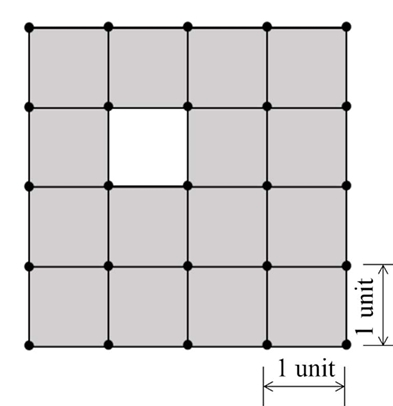
\includegraphics[width=0.3\columnwidth]{figs/fig-1.jpeg}
    \caption*{Fig-1:Grid of unit squares}
    \label{fig-1}
\end{figure}
What is the maximum number of squares without a "hole in the interior" that can be formed within the $4\times4$ grid using the unit squares as building blocks?
\newpage
\vspace*{0.25cm}
\begin{multicols}{4}
\begin{enumerate}
    \item $15$
    \item $20$
    \item $21$
    \item $26$
\end{enumerate}
\end{multicols}
\end{enumerate}

\begin{enumerate}[itemsep=1em]
\setcounter{enumi}{4}
\item An art gallery engages a security guard to ensure that the items displayed are protected. The diagram below represents the plan of the gallery where the boundary walls are opaque. The location the security guard posted is identified such that all the inner space (shaded region in the plan) of the gallery is within the line of sight of the security guard.\\
\\
If the security guard does not move around the posted location and has a $360\degree$view, which one of the following correctly represents the set of ALL possible locations among the locations P, Q, R and S, where the security guard can be posted to watch over the entire inner space of the gallery.  
\begin{figure}[H]
    \centering
    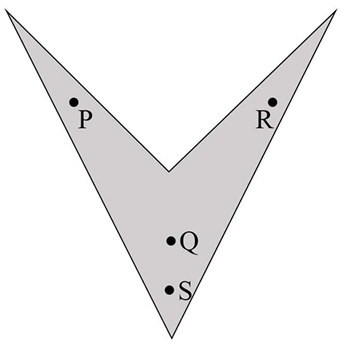
\includegraphics[width=0.3\columnwidth]{figs/fig-2.jpeg}
    \caption*{Fig-2:Plan of the art gallery}
    \label{fig-2}
\end{figure}
\begin{multicols}{4}
\begin{enumerate}
     \item P and Q
     \item Q
     \item Q and S
     \item R and S
\end{enumerate}
\end{multicols}
\end{enumerate}
\newpage
\vspace*{0.25cm}
\subsubsection{\underline{Q.6 \text{-} Q.10 Carry TWO mark Each}}
\setlength{\parskip}{1em}

\begin{enumerate}[itemsep=1em]
\setcounter{enumi}{5}
\item Mosquitoes pose a threat to human health. Controlling mosquitoes using chemicals may have undesired consequences. In Florida, authorities have used genetically modified mosquitoes to control the overall mosquito population. It remains to be seen if this novel approach has unforeseen consequences. \\
\\
Which one of the following is the correct logical inference based on the information in the above passage? 
\begin{enumerate}[leftmargin=2.5em, labelsep=0.5em, itemsep=0.5em]
    \item Using chemicals to kill mosquitoes is better than using genetically modified mosquitoes because genetic engineering is dangerous 
    \item Using genetically modified mosquitoes is better than using chemicals to kill mosquitoes because they do not have any side effects 
    \item Both using genetically modified mosquitoes and chemicals have undesired consequences and can be dangerous
    \item Using chemicals to kill mosquitoes may have undesired consequences but it is not clear if using genetically modified mosquitoes has any negative consequence 
\end{enumerate}
\end{enumerate}

\begin{enumerate}[itemsep=1em]
\setcounter{enumi}{6}
\item Consider the following inequalities. \\
      (i) $2x-1>7$\\
      (ii) $2x-1<9$\\
Which one of the following expressions below satisfies the above two inequalities? 
\begin{multicols}{4}
\begin{enumerate}
    \item $x \leq -4$
    \item $-4 < x \leq 4$
    \item $4<x<5$
    \item $x \geq 5$
\end{enumerate}    
\end{multicols}
\end{enumerate}

\begin{enumerate}[itemsep=1em]
\setcounter{enumi}{7}
\item Four points P(0,1), Q(0,-3), R(-2,-1),  and S(2,-1) represent the vertices of a quadrilateral.What is the area enclosed by the quadrilateral? 
\begin{multicols}{4}
\begin{enumerate}
    \item $4$
    \item $4\sqrt{2}$
    \item $8$
    \item $8\sqrt{2}$
\end{enumerate}
\end{multicols}
\end{enumerate}

\newpage
\vspace*{0.25cm}

\begin{enumerate}[itemsep=1em]
\setcounter{enumi}{8}
\item In a class of five students P, Q, R, S and T, only one student is known to have copied in the exam. The disciplinary committee has investigated the situation and recorded the statements from the students as given below.\\
\textbf{Statement of P}: R has copied in the exam. \\
\textbf{Statement of Q}: S has copied in the exam. \\
\textbf{Statement of R}: P did not copy in the exam. \\
\textbf{Statement of S}: Only one of us is telling the truth. \\
\textbf{Statement of T}: R is telling the truth. \\
The investigating team had authentic information that S never lies. Based on the information given above, the person who has copied in the exam is 
\begin{multicols}{4}
\begin{enumerate}
    \item R
    \item P
    \item Q
    \item T
\end{enumerate}
\end{multicols}
\end{enumerate}

\begin{enumerate}[itemsep=1em]
\setcounter{enumi}{9}
\item Consider the following square with the four corners and the center marked as P, Q, R, S and T respectively. \\
Let X,Y and Z represent the following operations: 

X: rotation of the square by 180 degree with respect to the 
S-Q axis.  \\
Y: rotation of the square by 180 degree with respect to the P-R axis.  \\
Z: rotation of the square by 90 degree clockwise with respect to the axis \;perpendicular, going into the screen and passing through the point T. \\
Consider the following three distinct sequences of operation (which are applied in the left to right order).\\ 
(1) XYZZ\\ 
(2) XY \\
(3) ZZZZ \\
Which one of the following statements is correct as per the information provided above?  
\begin{figure}[H]
    \centering
    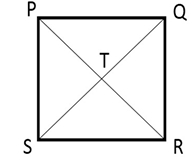
\includegraphics[width=0.2\columnwidth]{figs/fig-3.jpeg}
    \caption*{Fig-3}
    \label{fig-3}
\end{figure}

\begin{enumerate}[leftmargin=2.5em, labelsep=0.5em, itemsep=0.5em]
    \item The sequence of operations (1) and (2) are equivalent 
    \item The sequence of operations (1) and (3) are equivalent 
    \item The sequence of operations (2) and (3) are equivalent
    \item The sequence of operations (1), (2) and (3) are equivalent 
\end{enumerate}
\end{enumerate}
\newpage
\vspace*{0.25cm}
\subsubsection{\underline{Q.11 \text{-} Q.35 Carry ONE mark Each}}

\begin{enumerate}[itemsep=1em]
\setcounter{enumi}{10}
\item Let $A$ be a real non-zero square matrix of order n. If the homogeneous system of linear equations $Ax=0$ has only trivial solution, then 
\begin{enumerate}[leftmargin=2.5em, labelsep=0.5em, itemsep=0.5em]
    \item the matrix $A$ is singular
    \item the determinant of $A$ is zero 
    \item $\lambda=0$ is an eigenvalue of $A$
    \item for any n-vector $b$, the system of linear equations $Ax=b$ has a unique solution
\end{enumerate}
\end{enumerate}

\begin{enumerate}[itemsep=1em]
\setcounter{enumi}{11}
\item Let $z=x+iy$, where $x$ and $y$ are real numbers. Consider the complex functions: 
\[
f(z)=(x^2-y^2)\,+i\,2xy
\]
and
\[
g(z)=2xy\,+i\,(x^2-y^2)\,.
\]
Then on the complex plane, 
\begin{enumerate}[leftmargin=2.5em, labelsep=0.5em, itemsep=0.5em]
    \item $f(z)$ is analytic and $g(z)$ is not analytic
    \item both $f(z)$ and $g(z)$ are analytic 
    \item both $f(z)$ and $g(z)$ are not analytic 
    \item $f(z)$ is not analytic and $g(z)$ is analytic 
\end{enumerate}
\end{enumerate}

\begin{enumerate}[itemsep=1em]
\setcounter{enumi}{12}
\item If a population has exponential distribution with mean 1, then its median is  
\begin{multicols}{4}
\begin{enumerate}
    \item $e$
    \item 1
    \item $\log_e2$
    \item $\log_e3$
\end{enumerate}
\end{multicols}
\end{enumerate}

\begin{enumerate}[itemsep=1em]
\setcounter{enumi}{13}
\item Let $\omega_f$ be the excitation frequency of a sinusoidal load and $\omega_n$ be the natural frequency of a single degree of freedom system. Then the dynamic response of the system is highly affected by the stiffness of the system when 
\begin{multicols}{4}
\begin{enumerate}
    \item $\omega_f=\omega_n$
    \item $0<\omega_n<\omega_n$
    \item $0<\omega_n<\omega_f$
    \item $\omega_f=0$
\end{enumerate}
\end{multicols}
\end{enumerate}

\begin{enumerate}[itemsep=1em]
\setcounter{enumi}{14}
\item A truck loaded with a half-filled water tank is moving at a constant horizontal acceleration a. The acceleration due to gravity is g. At steady state, the angle $\theta$ made by the free surface with the horizontal plane is
\begin{multicols}{4}
\begin{enumerate}
    \item $\sin^{-1}(a/g)$
    \item $\tan^{-1}(g/a)$
    \item $\tan^{-1}(a/g)$
    \item $\sin^{-1}(g/a)$
\end{enumerate}
\end{multicols}
\end{enumerate}

\newpage
\vspace*{0.25cm}

\begin{enumerate}[itemsep=1em]
\setcounter{enumi}{15}
\item Which one of the following combinations of elementary flows will lead to an ideal flow past a deeply submerged circular cylinder with circulation?
\begin{enumerate}[leftmargin=2.5em, labelsep=0.5em, itemsep=0.5em]
    \item Source, sink and uniform flow 
    \item Doublet, uniform flow and vortex 
    \item Doublet and vortex 
    \item Source and uniform flow 
\end{enumerate}
\end{enumerate}

\begin{enumerate}[itemsep=1em]
\setcounter{enumi}{16}
\item A 10000 tonne displacement container ship's main propulsion engine has a brake power equal to 46 MW and its service speed is 25 knots. Considering the engine brake power as double the effective power of the ship, then the ship resistance at the service speed lies in between \underline{\hspace{2cm}} kN. 
\begin{multicols}{4}
\begin{enumerate}
    \item 3285 and 3315 
    \item 6785 and 6815 
    \item 885 and 915 
    \item 1785 and 1815 
\end{enumerate}   
\end{multicols}
\end{enumerate}

\begin{enumerate}[itemsep=1em]
\setcounter{enumi}{17}
\item The margin line used for the floodable length calculation of a ship is
\begin{enumerate}[leftmargin=2.5em, labelsep=0.5em, itemsep=0.5em]
    \item 76 mm above the ship's baseline 
    \item 76 mm inside the zero-buttock line in the profile view of the ship's lines plan 
    \item a line drawn 76 mm parallel to and below the watertight main deck at side 
    \item a line drawn 76 mm parallel to and below the watertight main deck along the ship's centerline if the ship has camber 
\end{enumerate}
\end{enumerate}

\begin{enumerate}[itemsep=1em]
\setcounter{enumi}{18}
\item Consider a rectangular box barge of length 80 m, breadth 20 m and depth 15 m floating at an even draught of 10 m. Assume that the heave added mass of the vessel is equal to its mass displacement and the acceleration due to gravity is 9.81 $m/s^2$. The heave natural period of the vessel lies in between \underline{\hspace{2cm}} s.
\begin{multicols}{4}
\begin{enumerate}
    \item 1 and 5
    \item 6 and 10 
    \item 11 and 15 
    \item 16 and 20 
\end{enumerate}  
\end{multicols}
\end{enumerate}

\begin{enumerate}[itemsep=1em]
\setcounter{enumi}{19}
\item A 1:20 scaled model of a surface ship is tested in a towing tank. The model is towed at 3 m/s and drag force measured is 10 N. The velocity of the prototype and the drag force acting on the prototype, respectively, are \underline{\hspace{1cm}} m/s and \underline{\hspace{1cm}} kN. 
\begin{multicols}{4}
\begin{enumerate}
    \item 60.4 and 80 
    \item 13.4 and 80 
    \item 13.4 and 4 
    \item 60.4 and 4 
\end{enumerate}   
\end{multicols}
\end{enumerate}
\newpage
\vspace*{0.25cm}
\begin{enumerate}[itemsep=1em]
\setcounter{enumi}{20}
\item In a diesel engine, the ignition is initiated by the 
\begin{enumerate}[leftmargin=2.5em, labelsep=0.5em, itemsep=0.5em]
    \item spark 
    \item preheating of the fuel 
    \item heating due to the compression of intake air 
    \item preheating of the intake air 
\end{enumerate}
\end{enumerate}

\begin{enumerate}[itemsep=1em]
\setcounter{enumi}{21}
\item In an internal combustion engine, supercharging is the process of supplying intake air at a pressure
\begin{enumerate}[leftmargin=2.5em, labelsep=0.5em, itemsep=0.5em]
    \item higher than that of the ambient 
    \item lower than that of the fuel 
    \item higher than that of the fuel 
    \item lower than that of the ambient 
\end{enumerate}
\end{enumerate}

\begin{enumerate}[itemsep=1em]
\setcounter{enumi}{22}
\item The most desirable property amongst the following for a lubricating oil is
\begin{enumerate}[leftmargin=2.5em, labelsep=0.5em, itemsep=0.5em]
    \item high density 
    \item high dynamic viscosity 
    \item low density
    \item low dynamic viscosity 
\end{enumerate}
\end{enumerate}

\begin{enumerate}[itemsep=1em]
\setcounter{enumi}{23}
\item If $\frac{a_0}{2}+\sum_{n=1}^{\infty}\,a_n\cos\,nx$  is the Fourier cosine series of the function $f(x)=\sin\,x\,,\;0<x<\pi,$ then which of the following are TRUE?  
\begin{multicols}{4}
\begin{enumerate}
    \item $a_0+a_1=4/\pi$
    \item $a_0=4/\pi$
    \item $a_0+a_1=2/\pi$
    \item $a_1=2/\pi$
\end{enumerate}    
\end{multicols}
\end{enumerate}

\begin{enumerate}[itemsep=1em]
\setcounter{enumi}{24}
\item A simply supported beam is loaded with a uniformly distributed load (UDL) acting 
vertically downwards. Which of the following statements are TRUE with regard to 
strain energy?  
\begin{enumerate}[leftmargin=2.5em, labelsep=0.5em, itemsep=0.5em]
    \item It increases with increase in UDL
    \item It increases with increase in cross-sectional area of the beam 
    \item It is independent of the length of the beam 
    \item It is dependent on Young's modulus of elasticity 
\end{enumerate}
\end{enumerate}

\newpage
\vspace*{0.25cm}

\begin{enumerate}[itemsep=1em]
\setcounter{enumi}{25}
\item Which of the following flows are represented by the velocity field,\\ $\overrightarrow{V} = (x^2-y^2)\,\hat{i} - 2xy\hat{j}$
\begin{enumerate}[leftmargin=2.5em, labelsep=0.5em, itemsep=0.5em]
    \item Incompressible flow 
    \item Compressible flow 
    \item Irrotational flow 
    \item Rotational flow 
\end{enumerate}    
\end{enumerate}

\begin{enumerate}[itemsep=1em]
\setcounter{enumi}{26}
\item If a ship enters shallow water from deep water, maintaining the same speed, then which of the following are TRUE? 
\begin{enumerate}[leftmargin=2.5em, labelsep=0.5em, itemsep=0.5em]
    \item Resistance increases 
    \item Trim changes 
    \item Resistance decreases 
    \item Draught increases 
\end{enumerate}
\end{enumerate}

\begin{enumerate}[itemsep=1em]
\setcounter{enumi}{27}
\item For a rigid vessel at sea, which of the following statements are TRUE?
\begin{enumerate}[leftmargin=2.5em, labelsep=0.5em, itemsep=0.5em]
    \item Static and dynamic environmental loads are dependent on the structural strength of the vessel 
    \item Static and dynamic environmental loads are NOT dependent on the structural strength of the vessel 
    \item Static and dynamic environmental loads are dependent on the geometry of the vessel 
    \item Static and dynamic environmental loads are NOT dependent on the geometry of the vessel 
\end{enumerate}
\end{enumerate}

\begin{enumerate}[itemsep=1em]
\setcounter{enumi}{28}
\item Which of the following are TRUE for pressure, temperature and density of a thermodynamic system?
\begin{enumerate}[leftmargin=2.5em, labelsep=0.5em, itemsep=0.5em]
    \item path functions 
    \item point functions 
    \item inexact differentials 
    \item exact differentials 
\end{enumerate}
\end{enumerate}

\begin{enumerate}[itemsep=1em]
\setcounter{enumi}{29}
\item Let $f(x,y,z)=xy+yz+xz$. If a point $(0,0,\lambda)$ lies on the tangent plane to the surface $f(x,y,z)=3$ at the point (1,1,1), then the value of $\lambda$ is \underline{\hspace{2cm}} . 
\end{enumerate}

\newpage
\vspace*{0.25cm}

\begin{enumerate}[itemsep=1em]
\setcounter{enumi}{30}
\item The beam fixed at end A and simply supported at C with a roller is shown in the figure. If B is an internal hinge and a concentrated load of 10 kN is acting at D and a uniformly distributed load (UDL) of 10 kN/m is acting on member AB, then the magnitude of bending moment at the fixed end A is \underline{\hspace{2cm}}  kNm. 
\begin{figure}[H]
    \centering
    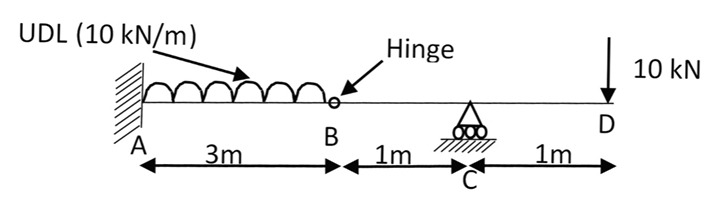
\includegraphics[width=0.6\columnwidth]{figs/fig-4.jpeg}
    \caption*{Fig-4}
    \label{fig-4}
\end{figure}

\end{enumerate}

\begin{enumerate}[itemsep=1em]
\setcounter{enumi}{31}
\item The laminar and turbulent boundary layer thickness of a flat plate are given by $\frac{5x}{Re_x^{1/2}}$ and $\frac{0.37x}{Re_x^{1/2}}$ , respectively, where $x$ is the distance from the leading edge and $Re_x$ is the Reynolds number at $x$-location. \\
\\
The kinematic viscosity of the fluid is $10^{-6}\, m^2/s$. A 100 m long plate is moving at a speed of 10 m/s.The boundary layer thickness at the rear end of the plate is \underline{\hspace{2cm}} m (rounded off to two decimal places)
\end{enumerate}

\begin{enumerate}[itemsep=1em]
\setcounter{enumi}{32}
\item he diameter and rotating speed of a cargo ship propeller are 7.5 m and 120 RPM, respectively.  An open water test is to be performed in a towing tank with a propeller model of 300 mm diameter. The corresponding propeller model speed is \underline{\hspace{2cm}} RPM. 
\end{enumerate}

\begin{enumerate}[itemsep=1em]
\setcounter{enumi}{33}
\item Assume that a ship has length L = 200 m and operates at a design speed U = 12 m/s. 
If in a turning circle maneuver, the ship exhibits a steady turning diameter of 6L,then the yaw rate of the ship is \underline{\hspace{2cm}} rad/s (correct to two decimal places). 
\end{enumerate}

\begin{enumerate}[itemsep=1em]
\setcounter{enumi}{34}
\item If the maximum static deflection of a shaft is 5 mm, then the estimated critical speed using Rayleigh-Ritz method is \underline{\hspace{2cm}} RPM (rounded off to nearest integer). 
\end{enumerate}

\newpage
\vspace*{0.25cm}

\subsubsection{\underline{Q.36 \text{-} Q.65 Carry TWO mark Each}}

\begin{enumerate}[itemsep=1em]
\setcounter{enumi}{35}
\item The value of the line integral 
\[
\oint_c -3y\,dx+3x\,dy+z\,dz
\]
along the circle $C:x^2+y^2=1,\, z=1$ oriented in the clockwise sense as seen from the origin, is
\begin{multicols}{4}
\begin{enumerate}
    \item $2\pi$
    \item $4\pi$
    \item $6\pi$
    \item $8\pi$
\end{enumerate}
\end{multicols}
\end{enumerate}

\begin{enumerate}[itemsep=1em]
\setcounter{enumi}{36}
\item A column of height 20 m is fixed at both ends. If Young's modulus of elasticity is $17\times 10^9$ N/m  and moment of inertia is $3.255\times 10^{-4}$ m, then the first critical load of buckling of the column lies between \underline{\hspace{2cm}} kN. 
\end{enumerate}

\begin{multicols}{4}
\begin{enumerate}
    \item 501 and 520 
    \item 521 and 540
    \item 541 and 560 
    \item 561 and 580 
\end{enumerate}
\end{multicols}

\begin{enumerate}[itemsep=1em]
\setcounter{enumi}{37}
\item In a potential flow field, if the stream function $\varphi=xy^2$, then the velocity potential $\phi$ is 
\begin{multicols}{4}
\begin{enumerate}
    \item $\frac{x^2-y^2}{2}$
    \item $\frac{x^2+y^2}{2}$
    \item $y\,(x^2+\frac{y^2}{3})$
    \item $y\,(x^2-\frac{y^2}{3})$
\end{enumerate}
\end{multicols}
\end{enumerate}

\begin{enumerate}[itemsep=1em]
\setcounter{enumi}{38}
\item For a container ship, the propeller open water efficiency, thrust deduction fraction and wake fraction are 0.60, 0.19 and 0.25, respectively. If the relative rotative efficiency of the propeller is 1.0, then the hull efficiency and quasi-propulsive efficiency of the propeller, respectively, are 
\begin{multicols}{4}
\begin{enumerate}
    \item 1.080 and 0.648
    \item 0.608 and 0.556 
    \item 0.926 and 0.648
    \item 0.926 and 0.556 
\end{enumerate}
\end{multicols}
\end{enumerate}

\begin{enumerate}[itemsep=1em]
\setcounter{enumi}{39}
\item Consider the wave elevation spectrum $S_{\eta\eta}(\omega)$ as shown in the figure. Then, the significant wave height is \underline{\hspace{1cm}} m.
\begin{figure}[H]
    \centering
    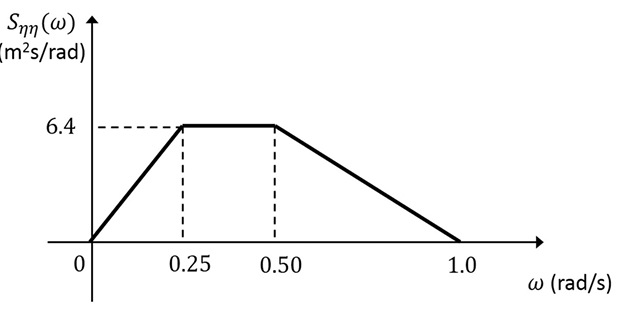
\includegraphics[width=0.3\columnwidth]{figs/fig-5.jpeg}
    \caption*{Fig-5:Wave elevation spectrum}
    \label{fig-5}
\end{figure}
\begin{multicols}{4}
\begin{enumerate}
    \item 2
    \item 4
    \item 6
    \item 8
\end{enumerate}    
\end{multicols}
\end{enumerate}

\newpage
\vspace*{0.25cm}

\begin{enumerate}[itemsep=1em]
\setcounter{enumi}{40}
\item If $\Delta h_m$ and $\Delta h_f$ are the enthalpy drops across the moving and fixed blades of a turbine stage, then the degree of reaction is 
\begin{multicols}{4}
\begin{enumerate}
    \item $\frac{\Delta h_m}{\Delta h_f}$
    \item $\frac{\Delta h_f}{\Delta h_m}$
    \item $\frac{\Delta h_m}{\Delta h_m + \Delta h_f}$
    \item $\frac{\Delta h_f}{\Delta h_m + \Delta h_f}$
\end{enumerate}
\end{multicols}
\end{enumerate}

\begin{enumerate}[itemsep=1em]
\setcounter{enumi}{41}
\item Let M=$\begin{myvec}{2&&-1&&1 \\ -1&&2&&-1 \\ 1&&-1&&2}\end{myvec}$ .Which of the following are TRUE?

\begin{enumerate}[leftmargin=2.5em, labelsep=0.5em, itemsep=0.5em]
    \item M is singular
    \item $M^{-1}=\frac{1}{4}M^2-\frac{3}{2}M+\frac{9}{4}I$, where $I$ is the identity matrix of order 3 
    \item $M$ has three distinct eigenvalues 
    \item $M$ has three linearly independent eigenvectors 
\end{enumerate}
\end{enumerate}


\begin{enumerate}[itemsep=1em]
\setcounter{enumi}{42}
\item Which of the following statements are TRUE about the assumptions adopted in Euler's column theory? 
\begin{enumerate}[leftmargin=2.5em, labelsep=0.5em, itemsep=0.5em]
    \item Length of the column is very large in comparison to its cross-sectional dimensions
    \item Effect of the axial compressive stress is smaller than the effect of bending stress on column buckling
    \item Column fails only by transverse loads 
    \item Column fails only by buckling 
\end{enumerate}
\end{enumerate}

\begin{enumerate}[itemsep=1em]
\setcounter{enumi}{43}
\item An autonomous underwater vehicle is made of a long cylinder with a semi-ellipsoid at the forward end and a hemisphere at the aft end as shown in the figure. The origin of the reference frame is located at the centroid of the cylinder. \\
\\
The positive x, y and z axes, respectively, are pointing towards forward, port and upward directions. The surge, sway and heave motions are represented by indices 1-2-3 and roll, pitch and yaw motions are represented by indices 4-5-6, respectively. \\
\\
If $A=[A_{ij}]$ is the added mass matrix, then which of the following are NOT zero? 
\begin{figure}[H]
    \centering
    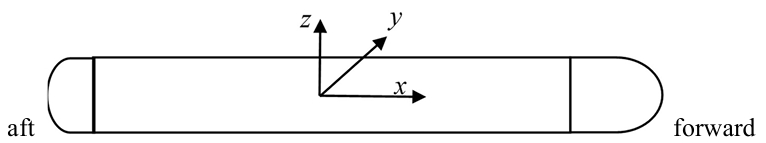
\includegraphics[width=0.4\columnwidth]{figs/fig-6.jpeg}
    \caption*{Fig-6:Autonomous underwater vehicle}
    \label{fig-6}
\end{figure}
\newpage
\vspace*{0.25cm}
\begin{multicols}{4}
\begin{enumerate}
    \item $A_{15}$
    \item $A_{35}$
    \item $A_{46}$
    \item $A_{26}$
\end{enumerate}
\end{multicols}
\end{enumerate}

\begin{enumerate}[itemsep=1em]
\setcounter{enumi}{44}
\item If a ship hull is subdivided into different watertight compartments, which of the following statements are TRUE? 
\begin{enumerate}[leftmargin=2.5em, labelsep=0.5em, itemsep=0.5em]
    \item It improves the ship stability in damaged conditions 
    \item It increases the ship hull strength 
    \item It reduces the ship intact stability 
    \item It provides more options to carry different types of cargo 
\end{enumerate}
\end{enumerate}


\begin{enumerate}[itemsep=1em]
\setcounter{enumi}{45}
\item Consider the midship section of a vessel with the centerline (CL) and neutral axis (NA) as shown in the figure. Assume that the cross-section is symmetric about the centerline, the plate thickness is uniform throughout the section and $h_1<h_2$.\\
\\
When the vessel is subjected to a vertical bending moment in its upright condition, which of the following statements are TRUE?
\begin{figure}[H]
    \centering
    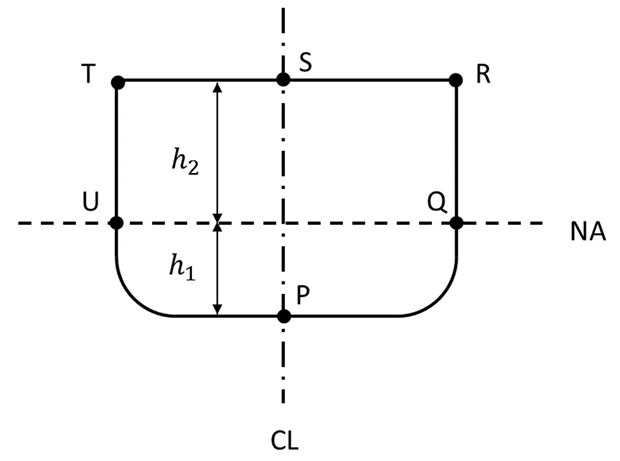
\includegraphics[width=0.4\columnwidth]{figs/fig-7.jpeg}
    \caption*{Fig-7:midship section of the vessel}
    \label{fig-7}
\end{figure}
\begin{enumerate}[leftmargin=2.5em, labelsep=0.5em, itemsep=0.5em]
    \item Magnitude of shear stress is maximum at points P and S 
    \item Magnitude of shear stress is minimum at points Q and U 
    \item Magnitude of bending stress is maximum at points S and T 
    \item Magnitude of bending stress is minimum at points Q and U 
\end{enumerate}
\end{enumerate}

\newpage
\vspace*{0.25cm}

\begin{enumerate}[itemsep=1em]
\setcounter{enumi}{46}
\item For a simple vapour compression refrigeration, which of the following thermodynamic cycles (1-2-3-4) are possible? Here,$T,P,s\;and\,h$ indicate temperature,pressure,specific entropy and specific enthalpy, respectively.
\begin{multicols}{4}
\begin{enumerate}
    \item \begin{minipage}[t]{0.2\textwidth}
    \vspace{0pt}
        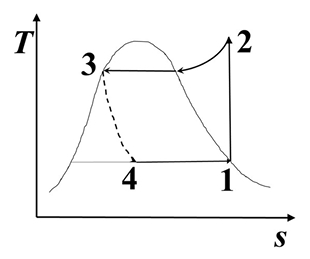
\includegraphics[width=\columnwidth]{figs/fig-8.jpeg}
        \label{fig-11}
    \end{minipage}
    \item \begin{minipage}[t]{0.2\textwidth}
    \vspace{0pt}
        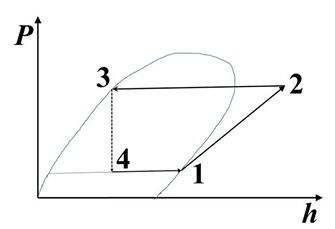
\includegraphics[width=\columnwidth]{figs/fig-9.jpeg}
        \label{fig-12}
    \end{minipage}
    \item \begin{minipage}[t]{0.2\textwidth}
    \vspace{0pt}
        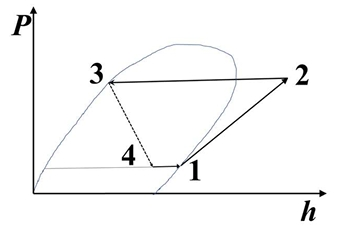
\includegraphics[width=\columnwidth]{figs/fig-10.jpeg}
        \label{fig-13}
    \end{minipage}
    \item \begin{minipage}[t]{0.2\textwidth}
    \vspace{0pt}
        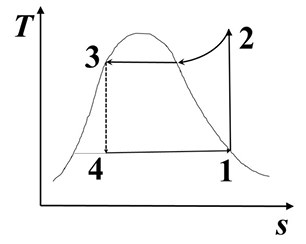
\includegraphics[width=\columnwidth]{figs/fig-11.jpeg}
    \label{fig-14}
    \end{minipage}
\end{enumerate}
\end{multicols}
\end{enumerate}

\begin{enumerate}[itemsep=1em]
\setcounter{enumi}{47}
\item Which of the following statements are TRUE for a fluid flow over a deeply submerged body?
\begin{enumerate}[leftmargin=2.5em, labelsep=0.5em, itemsep=0.5em]
    \item D'Alembert's paradox states that a deeply submerged body in a real fluid flow experiences no drag force
    \item D'Alembert's paradox states that a deeply submerged body in an ideal fluid flow experiences no drag force 
    \item The wall shear stress at the point of flow separation on the body is zero 
    \item Dimples/dentures on a body surface facilitate earlier transition to turbulent flow which delays the boundary layer separation 
\end{enumerate}
\end{enumerate}

\begin{enumerate}[itemsep=1em]
\setcounter{enumi}{48}
\item An Otto cycle has states 1 and 2 at the beginning and the end of the compression stroke, respectively. The states 3 and 4 are at the beginning and the end of the expansion stroke, respectively. \\
\\
Let the compression ratio of the cycle be $r$, specific heat ratio of air be $\gamma$ , specific heat of air at constant volume be $C_v$,  and  P, $v$,  and T be pressure, specific volume and temperature of the air, respectively.  Then, which of the following expressions represent the thermal efficiency of the cycle? 
\begin{enumerate}[leftmargin=2.5em, labelsep=0.5em, itemsep=0.5em]
    \item $1-\frac{1}{r^{\gamma -1}}$
    \item $1-\frac{T_3-T_4}{T_2-T_1}$
    \item $\frac{(P_3v_3-P_4v_4)-(P_2v_2-P_1v_1)}{C_v(T_3-T_2)(\gamma -1)}$
    \item $1-r^{\gamma-1}$
\end{enumerate}
\end{enumerate}
\newpage
\vspace*{0.25cm}
\begin{enumerate}[itemsep=1em]
\setcounter{enumi}{49}
\item Let $y(x)$ be the solution of the differential equation  
\[
y''-4y'-12y=3e^{5x}
\]
satisfying $y(0)=\frac{18}{7}$ and $y'(0)=-\frac{1}{7}$\\
Then $y(1)$ is \underline{\hspace{1cm}} (rounded off to nearest integer). 
\end{enumerate}

\begin{enumerate}[itemsep=1em]
\setcounter{enumi}{50}
\item We have two coins. One is biased with the probability for head being 1.0 and the other is a fair coin.  One coin is chosen at random and is tossed twice. If we obtain head both times, then the probability of the chosen coin being a fair coin is \underline{\hspace{1cm}} (correct to one decimal place). 
\end{enumerate}

\begin{enumerate}[itemsep=1em]
\setcounter{enumi}{51}
\item An element, as shown in the figure, is subjected to stresses $\sigma_x= 500\,N/m^2$ , $\sigma_y=300\,N/m^2$ and $\tau=120\,N/m^2$.If $\sigma_1$ and $\sigma_2$ are the principal stresses, then the absolute value of the angle $\varphi$ is \underline{\hspace{1cm}} degree (rounded off to one decimal place).
\begin{figure}[H]
    \centering
    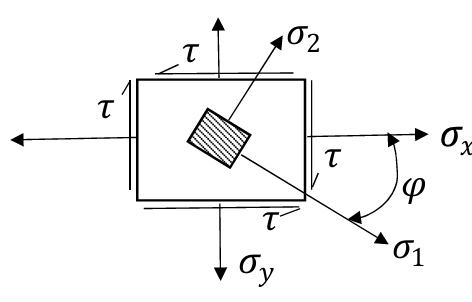
\includegraphics[width=0.4\columnwidth]{figs/fig-12.jpeg}
    \caption*{Fig-12:Element}
    \label{fig-12}
\end{figure}

\end{enumerate}

\begin{enumerate}[itemsep=1em]
\setcounter{enumi}{52}
\item An under-damped single degree of freedom system is freely oscillating with an initial amplitude $A$. The initial velocity of the system is zero.  After five cycles of oscillation, the amplitude reduces to $A/2$.Then the damping ratio of the system is \underline{\hspace{1cm}} \% (rounded off to one decimal place) of critical damping. 
\end{enumerate}

\begin{enumerate}[itemsep=1em]
\setcounter{enumi}{53}
\item A system with two degrees of freedom, as shown in the figure, has masses $m_1=200$ kg and  $m_2=100$ kg and stiffness coefficients $k_1=k_2=200$ N/m.  \\
Then the lowest natural frequency of the system is \underline{\hspace{1cm}} rad/s (rounded off to one decimal place).
\begin{figure}[H]
    \centering
    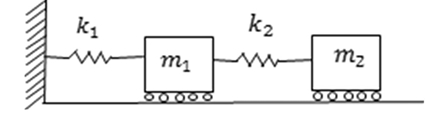
\includegraphics[width=0.4\columnwidth]{figs/fig-13.jpeg}
    \caption*{Fig-13}
    \label{fig-13}
\end{figure}
\end{enumerate}

\newpage
\vspace*{0.25cm}

\begin{enumerate}[itemsep=1em]
\setcounter{enumi}{54}
\item A horizontal cylinder of 1.0 m diameter is placed transversely at the aft of a ship and is completely immersed in water. The cylinder rotates at 100 RPM and inflow velocity is 10 m/s. Water density is $1000\, kg/m^3$. Assuming an ideal planar flow, the lift force/unit length acting on the cylinder is \underline{\hspace{1cm}} kN/m (rounded off to one decimal place). 
\end{enumerate}

\begin{enumerate}[itemsep=1em]
\setcounter{enumi}{55}
\item Consider a steady flow through a horizontal nozzle. The nozzle inlet area is $1 \,m^2$ and the outlet area is $0.05 \,m^2$. At the outlet, the flow discharges to atmosphere.Assuming the flow to be incompressible and frictionless, and the density of the fluid as $1\, kg/m^3$, the gauge pressure required at the nozzle inlet to produce an outlet speed of 100 m/s is \underline{\hspace{1cm}} (rounded off to the nearest integer)
\end{enumerate}

\begin{enumerate}[itemsep=1em]
\setcounter{enumi}{56}
\item A rectangular barge has length (L) of 100 m, breadth (B) of 18 m and depth (D) of 10 m. It is subdivided transversely into four equal compartments of equal length with the end compartments loaded fully with oil of density = $0.9\, tonne/m^3$.The barge floats in water having a density of $1000\, kg/m^3$. If the hull structural weight is ignored, then the transverse metacentric height of the barge is \underline{\hspace{1cm}} m (correct to two decimal places)
\begin{figure}[H]
    \centering
    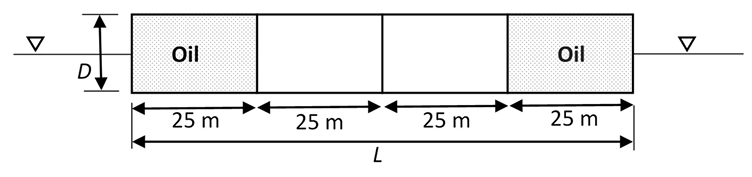
\includegraphics[width=0.4\columnwidth]{figs/fig-14.jpeg}
    \caption*{Fig-14:Rectangular barge}
    \label{fig-14}
\end{figure}
\end{enumerate}
\begin{enumerate}[itemsep=1em]
\setcounter{enumi}{57}
\item A propeller rotating at a speed of 108 RPM behind the ship produces a thrust of 720 kN with a torque of 700 kNm, when it travels at a speed of 15 knots. In open water, this propeller rotating at the same speed, produces the same thrust at an advance speed of 12 knots, and develops the same torque at an advance speed of 12.3 knots. Then, the average of the wake fractions is \underline{\hspace{1cm}}(correct to two decimal spaces)
\end{enumerate}
\newpage
\vspace*{0.25cm}

\begin{enumerate}[itemsep=1em]
\setcounter{enumi}{58}
\item Consider a point source in a uniform flow of velocity U=4 m/s along the positive $x$-axis as shown in the figure. Assume a two-dimensional steady potential flow. The potential due to the point source is given by $\log_e(r)$, where $r^2=x^2+y^2$ .  \\
\\
Then the magnitude of the distance $d$ between the point source and the stagnation point is \underline{\hspace{2cm}} m (rounded off to two decimal places). 
\begin{figure}[H]
    \centering
    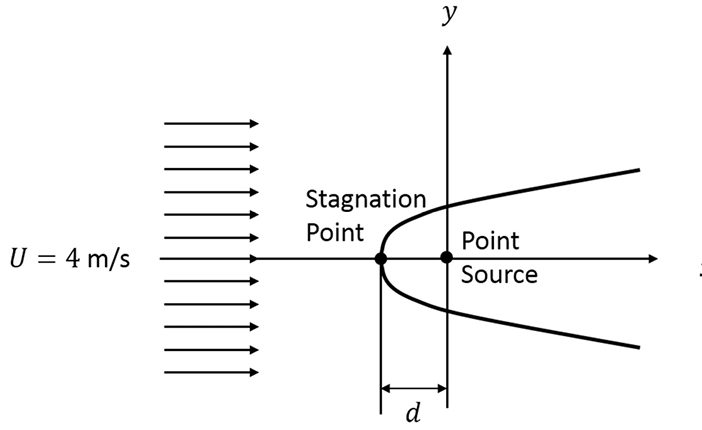
\includegraphics[width=0.4\columnwidth]{figs/fig-15.jpeg}
    \caption*{Fig-15:Two dimensional steady potential flow}
    \label{fig-15}
\end{figure}
\end{enumerate}

\begin{enumerate}[itemsep=1em]
\setcounter{enumi}{59}
\item Consider a ship with one half of its midship cross-section, as shown in the figure, with moulded breadth B of 30 m and moulded depth D of 9 m. \\ 
Assume the following: \\
\begin{itemize}[leftmargin=2.5em, labelsep=0.5em, itemsep=0.5em]
    \item The deck, side shell and bottom plate have the same thickness
    \item The yield stress of the material is 240 MPa
    \item The section is subjected to a vertical bending moment of 712.8 MNm
\end{itemize}

Ignore the self-moment of inertia of the deck and bottom plating in calculations.The distance of the fiber farthest from the neutral axis can be considered excluding the plate thickness. \\
\\
If the maximum bending stress is equal to the yield stress, then the plate thickness is \underline{\hspace{1cm}} mm (rounded off to one decimal place).

\begin{figure}[H]
    \centering
    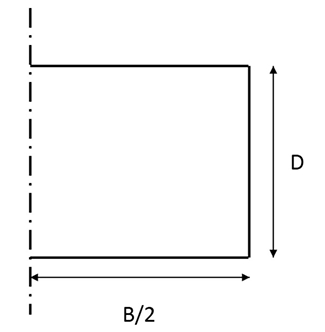
\includegraphics[width=0.2\columnwidth]{figs/fig-16.jpeg}
    \caption*{Fig-16: Mid-ship cross section of a ship}
    \label{fig-16}
\end{figure}
\end{enumerate}
\newpage
\vspace*{0.25cm}

\begin{enumerate}[itemsep=1em]
\setcounter{enumi}{60}
\item Consider a ship with a forward speed U of  9.81 m/s moving in deep waters. A wave is incident at an angle $\beta=120\degree$ to the longitudinal axis of the ship as shown in figure. Assume acceleration due to gravity g =9.81 m/s2. If a person onboard the ship observes the encounter period of the incident wave to be 4.187 s, then the actual period of the wave is \underline{\hspace{1cm}} s (rounded off to one decimal place). 
\begin{figure}[H]
    \centering
    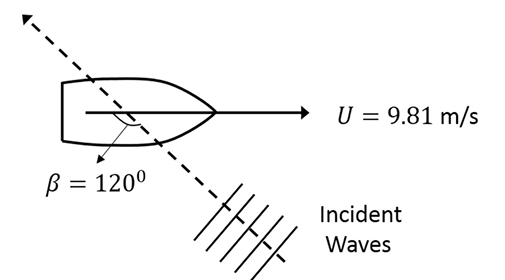
\includegraphics[width=0.2\columnwidth]{figs/fig-17.jpeg}
    \caption*{Fig-17}
    \label{fig-17}
\end{figure}
\end{enumerate}

\begin{enumerate}[itemsep=1em]
\setcounter{enumi}{61}
\item An air standard Otto cycle has a compression ratio of 6 and a mean effective pressure of 1000 kPa. Assume that the specific heat ratio $\gamma$ as 1.4 and specific gas constant $R$ as 0.287 kJ/kgK for the air. If the pressure and temperature at the beginning of the compression stroke are 100 kPa and 300 K, respectively, then the specific work output of the cycle is \underline{\hspace{2cm}} kJ/kg (rounded off to one decimal 
place). 
\end{enumerate}

\begin{enumerate}[itemsep=1em]
\setcounter{enumi}{62}
\item If methane $(CH_4)$ gas reacts with air at a stoichiometric proportion, then the air fuel ratio of the combustion process is \underline{\hspace{1cm}} (rounded off to one decimal place). 
\end{enumerate}

\begin{enumerate}[itemsep=1em]
\setcounter{enumi}{63}
\item In a vapour compression refrigeration cycle using R134 as the refrigerant, the enthalpies are (i) 240 kJ/kg at the beginning of the compression, (ii) 275 kJ/kg at the end of the compression and (iii) 96 kJ/kg at the beginning of the throttling. \\
\\
Then the coefficient of performance of the cycle is \underline{\hspace{2cm}} (rounded off to one decimal place). 
\end{enumerate}

\begin{enumerate}[itemsep=1em]
\setcounter{enumi}{64}
\item Consider a steady incompressible laminar flow between two parallel long plates separated by a distance $h$=1 m as shown in the figure. The bottom plate is fixed, and the flow is driven by the motion of the upper plate alone. No externally imposed pressure exists. \\
\\
If the upper plate has a velocity of U=10 m/s, the kinematic viscosity of the fluid is $10^{-6}\, m^2/s$ and the density of the fluid is $10^3 \,kg/m^3$, then the shear stress at the bottom plate is \underline{\hspace{1cm}} $N/m^2$ (correct to two decimal places) 
\begin{figure}[H]
    \centering
    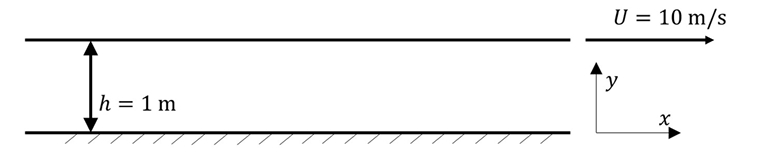
\includegraphics[width=0.4\columnwidth]{figs/fig-18.jpeg}
    \caption*{Fig-18:incompressible laminar flow between two long plates}
    \label{fig-17}
\end{figure}
\end{enumerate}


\end{document}
